\subsection{Alert}
Gli alert, conosciuti anche come allarmi, costituiscono notifiche inviate agli utenti per segnalare eventuali problemi o situazioni di criticità rilevate dai sensori.\\
Essi vengono generati in risposta al superamento di una soglia di allarme predefinita da parte di un evento. \\

\subsubsection{Visualizzazione degli Alert}
Gli alert vengono mostrati in un riquadro dedicato nella \textit{dashboard}\textsubscript{\textit{G}} principale, come mostrato nella sottosezione relativa alle tipologie dei grafici (\S~\ref{subsec:tipologie_grafici}). \\

\paragraph{Alert nei grafici}
In alcuni pannelli è possibile vedere gli alert direttamente nei grafici. In particolare è possibile visualizzare gli alert nei grafici a linee come una linea tratteggiata verticale che indica il punto nel tempo in cui l'alert è stato attivato. \\
\begin{figure}[H]
    \centering
    \fbox{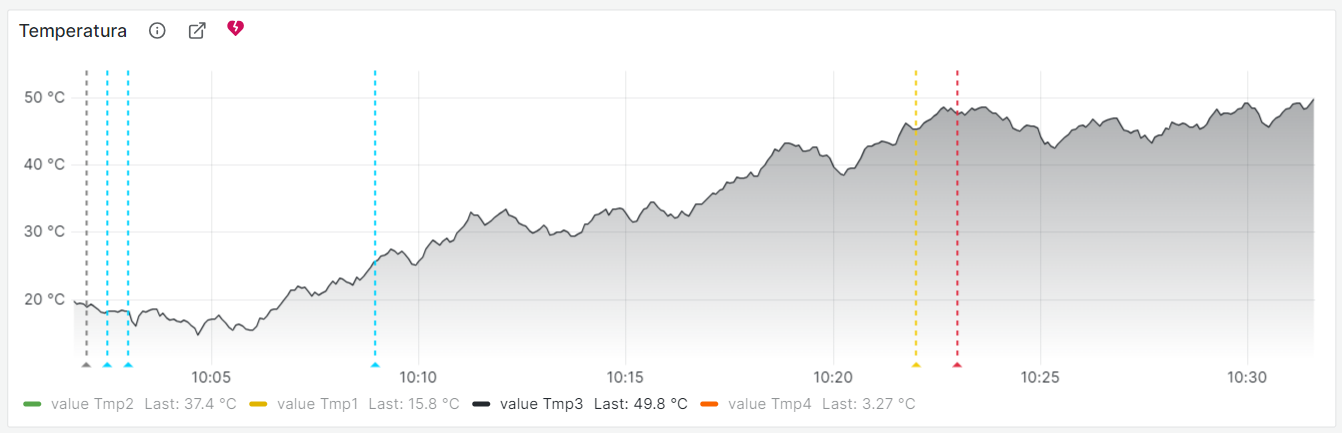
\includegraphics[width=12cm]{../Images/ManualeUtente/Light/panel_singolo_grafico.png}}
    \caption{Esempio di alert in un grafico a linee}
    \label{fig:my_label}
\end{figure}
Come si può notare dall'immagine sopra, in alto a sinistra è presente un'icona a forma di cuore che indica lo stato dell'alert del grafico. Può essere di tre tipi: 

\begin{itemize}
    \item \textbf{Ok}: l'icona rappresenta un cuore intero e non è presente alcuna linea tratteggiata nel grafico; 
    \begin{figure}[H]
        \centering
        \fbox{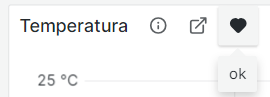
\includegraphics[width=4cm]{../Images/ManualeUtente/Light/alert_pannello_cuore_ok.png}}
        \caption{Stato "ok" dell'alert}
        \label{fig:my_label}
    \end{figure}
    \item \textbf{Alert pending}: 
    quando una condizione per l'attivazione dell'avviso è stata soddisfatta, ma il periodo di valutazione dell'avviso non è ancora trascorso. Il periodo di valutazione negli alert è il lasso di tempo durante il quale il \textit{sistema}\textsubscript{\textit{G}} verifica continuamente se una condizione di allarme è soddisfatta.  
    \begin{figure}[H]
        \centering
        \fbox{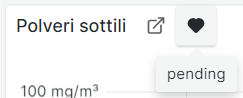
\includegraphics[width=4cm]{../Images/ManualeUtente/Light/alert_pannello_cuore_pending.png}}
        \caption{Stato "pending" dell'alert}
        \label{fig:my_label}
    \end{figure}
    \item \textbf{Alert attivo}: quando una condizione di attivazione dell'avviso è stata soddisfatta e il periodo di valutazione dell'avviso è trascorso. Come specificato nel punto precedente, il periodo di valutazione negli alert è il lasso di tempo durante il quale il \textit{sistema}\textsubscript{\textit{G}} verifica continuamente se una condizione di allarme è soddisfatta.   
    \begin{figure}[H]
        \centering
        \fbox{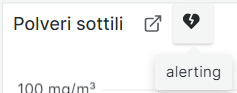
\includegraphics[width=4cm]{../Images/ManualeUtente/Light/alert_pannello_cuore_alerting.png}}
        \caption{Stato "alerting" dell'alert}
        \label{fig:my_label}
    \end{figure}
\end{itemize}

\paragraph{Ricezione notifiche alert}
É reso disponibile agli utenti un server \textit{Discord}\textsubscript{\textit{G}} dedicato per ricevere le notifiche degli alert in tempo reale. \\


\subsubsection{Server Discord}

\paragraph{Accesso al server Discord}
Qualora l'utente non fosse già iscritto a \textit{Discord}\textsubscript{\textit{G}}, è necessario creare un \textit{account}\textsubscript{\textit{G}} seguendo le istruzioni fornite dal sito ufficiale di Discord: \url{https://discord.com/}~(Consultato:~09/03/2024). \\
Per poter accedere al server dedicato, è necessario seguire i seguenti passaggi:
\begin{enumerate}
    \item Accedere al server tramite il \textit{link}\textsubscript{\textit{G}} del server InnovaCity: \url{https://discord.gg/9VZ8me7x}~(Consultato:~09/03/2024);
    \item Eseguire l'accesso al proprio \textit{account}\textsubscript{\textit{G}} o, nel caso non se ne fosse in possesso, creare un nuovo \textit{account}\textsubscript{\textit{G}};
    \begin{figure}[H]
        \centering
        \fbox{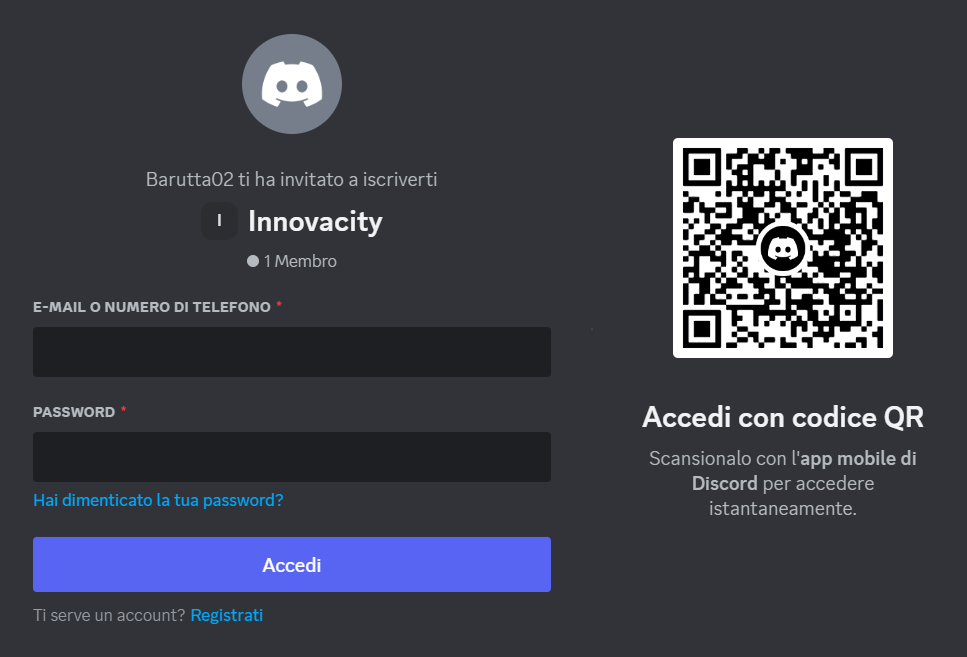
\includegraphics[width=9cm]{../Images/ManualeUtente/Light/accesso_discord.png}}
        \caption{Esempio di pagina login Discord}
        \label{fig:my_label}
    \end{figure}
    \item Una volta entrati nel server, sarà possibile visualizzare le notifiche degli alert in tempo reale nella sezione Informazioni/allerte. 
    \begin{figure}[H]
        \centering
        \fbox{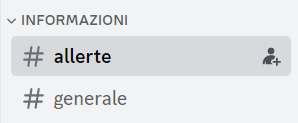
\includegraphics[width=4.5cm]{../Images/ManualeUtente/Light/canale_testuale.png}}
        \caption{Sezione del server Discord dedicata alle notifiche degli alert}    
        \label{fig:my_label}
    \end{figure}
\end{enumerate}

\paragraph{Ricezione delle notifiche su Discord}
Una volta entrati nel server \textit{Discord}\textsubscript{\textit{G}} sarà possibile ricevere le notifiche degli alert in tempo reale. Le notifiche vengono inviate in automatico dal \textit{sistema}\textsubscript{\textit{G}} e sono visibili nella sezione "informazioni/alert" del server \textit{Discord}\textsubscript{\textit{G}}. \\
Gli alert verranno mostrati nel seguente formato:
\begin{figure}[H]
    \centering
    \fbox{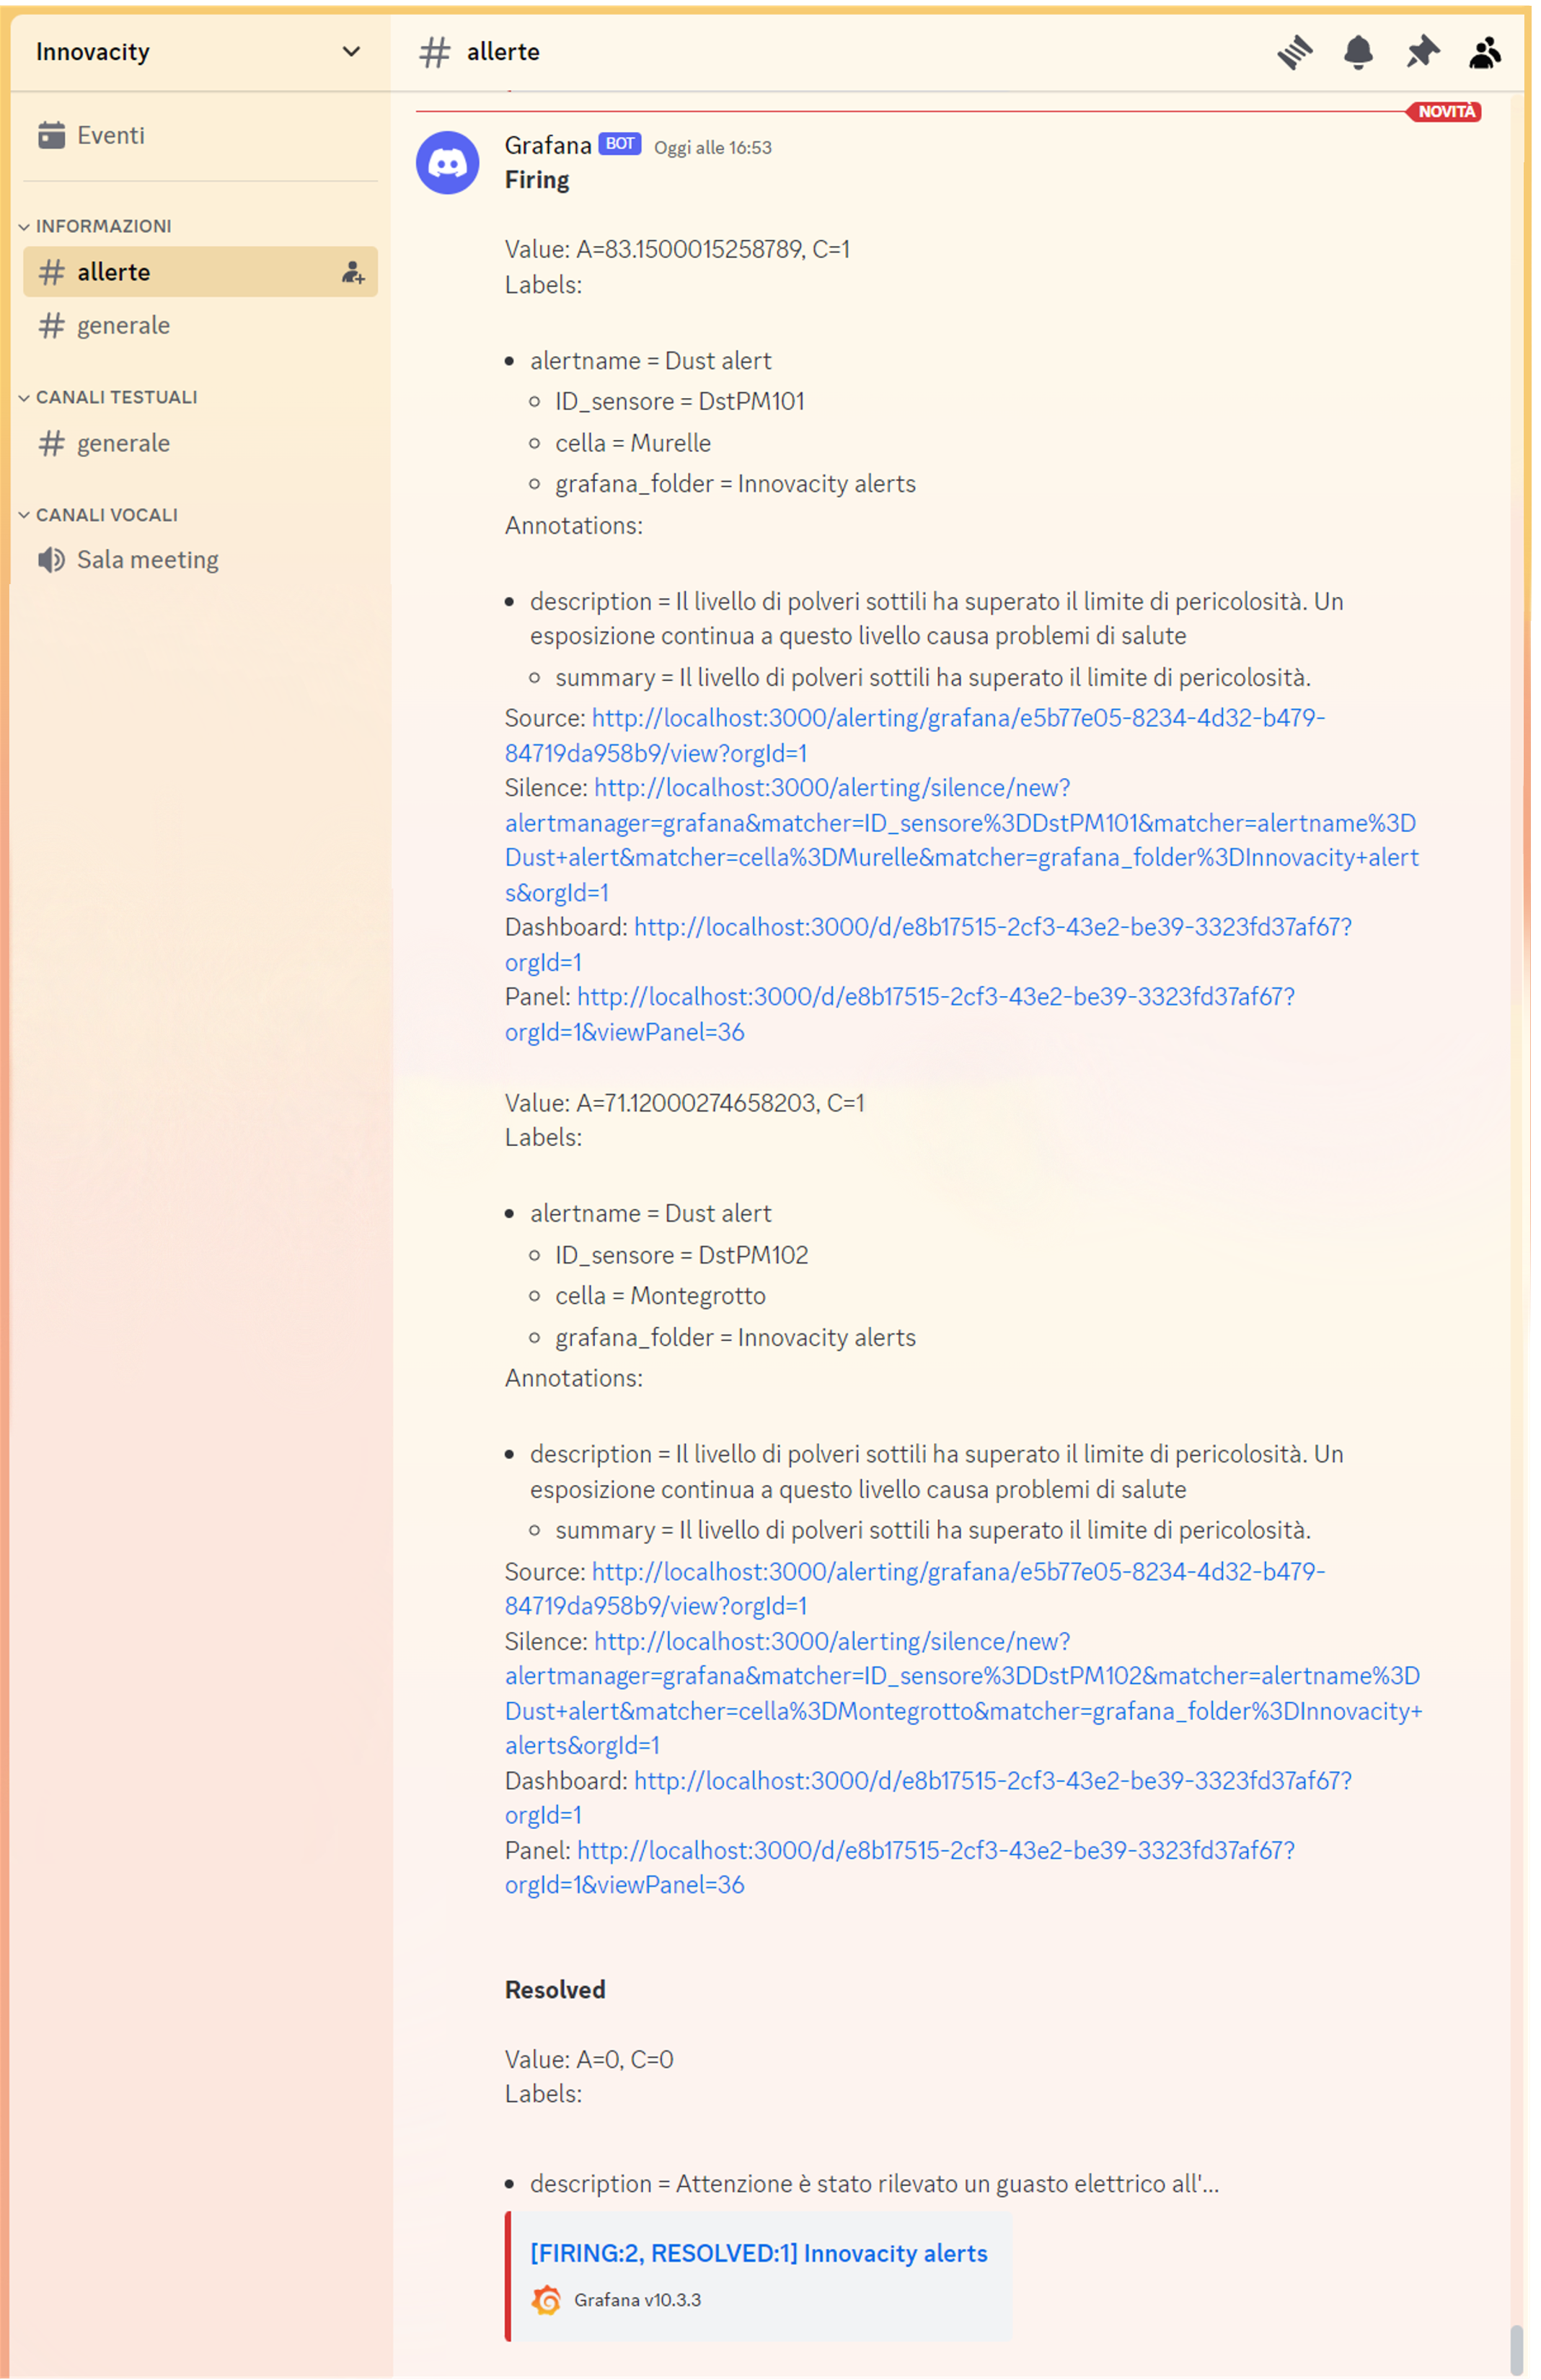
\includegraphics[width=8cm]{../Images/ManualeUtente/Light/discord_notification.png}}
    \caption{Esempio di notifica di un alert su Discord}
    \label{fig:my_label}
\end{figure} 